\begin{figure}[htbp]
  \centering

  \begin{subfigure}{0.48\textwidth}
    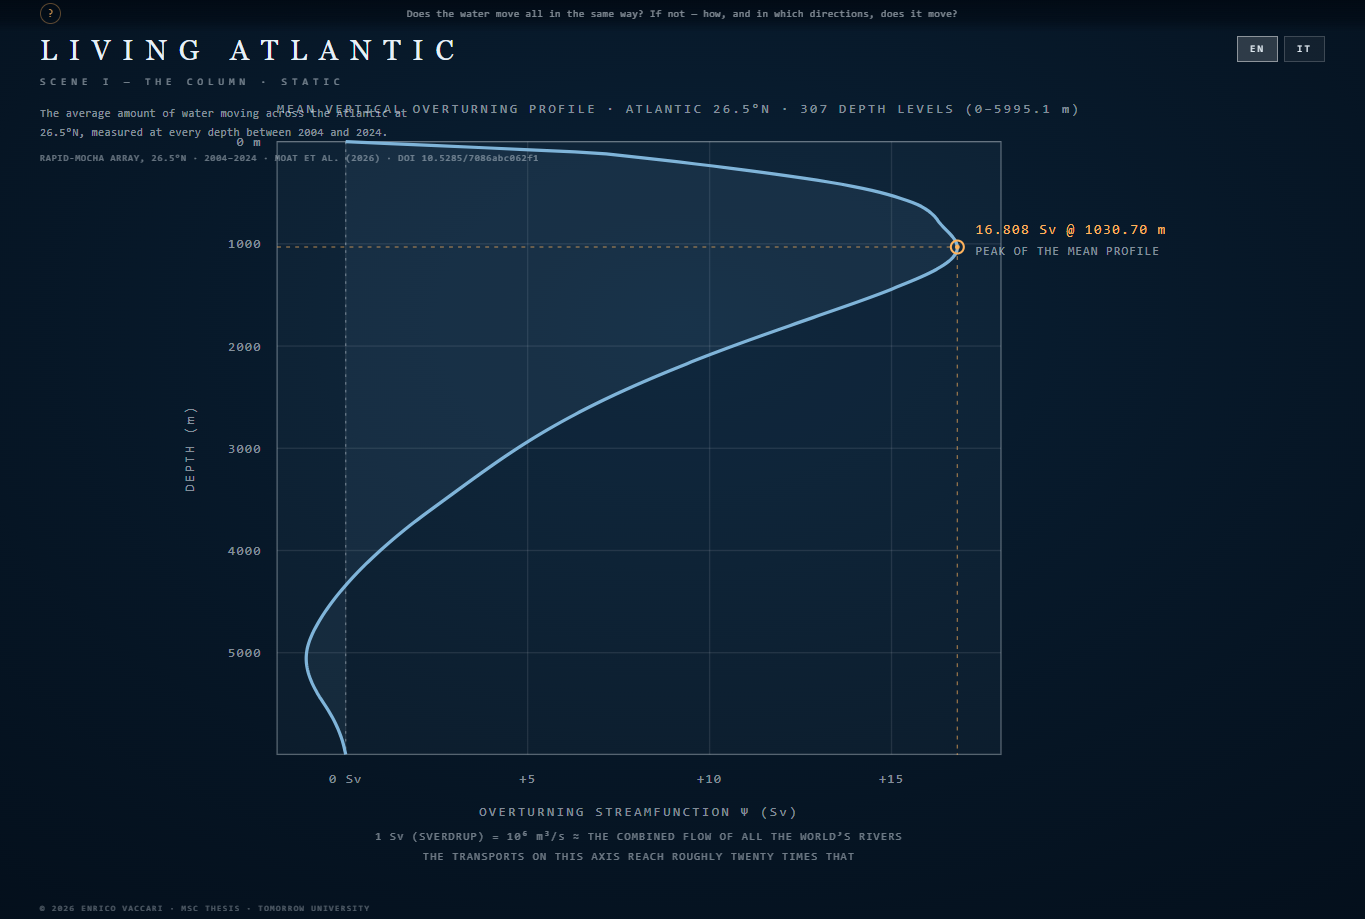
\includegraphics[width=\textwidth]{figures/viz1/viz1_thecolumn-static.png}
    \caption{Control (C1): the canonical static profile.}
    \label{fig:thecolumn-static}
  \end{subfigure}
  \hfill
  \begin{subfigure}{0.48\textwidth}
    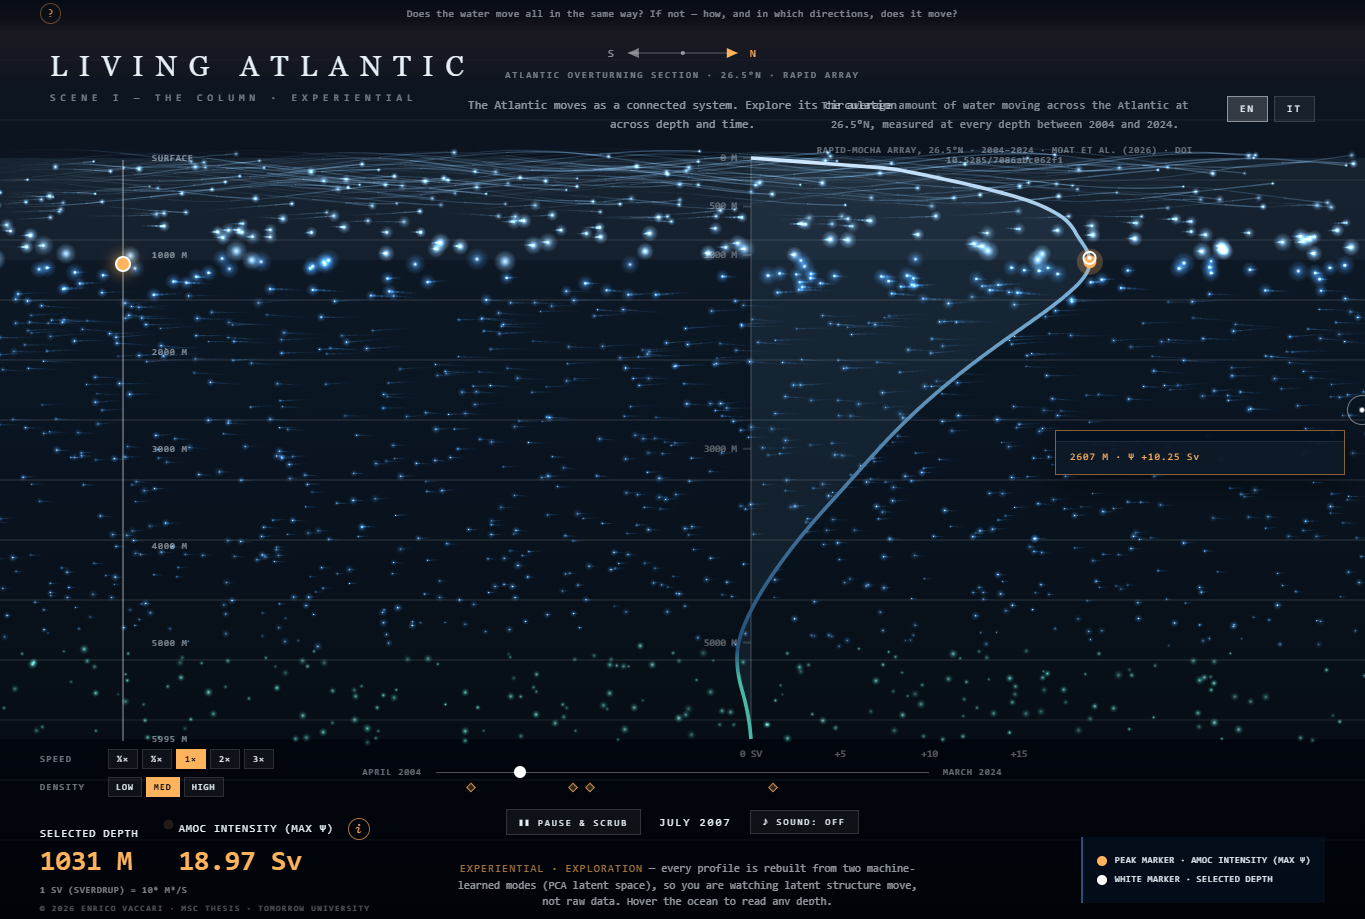
\includegraphics[width=\textwidth]{figures/viz1/viz1_thecolumn-experiential.png}
    \caption{Experiential (C2+C3): the same column set in motion.}
    \label{fig:thecolumn-experiential}
  \end{subfigure}

  \caption[The two conditions of Scene~I]{The two administered conditions of
  Scene~I, generated from the same data bundle through the same reconstruction
  function. The experiential condition introduces temporal behaviour while
  preserving the underlying structure of the static representation.}

  \label{fig:thecolumn-conditions}
\end{figure}